\chapter{Results}
This chapter includes the results of the survey study (chapter \ref{ch:survey}) and the experiments with the value-sensitive rejector (chapter \ref{ch:rejector}).
%
We first present the results of the survey study as the experiments with the value-sensitive rejector depended on the outcomes of the survey study.
%

%
The goal of the survey study was to retrieve the value ratios of TP, TN, FP, FN, and rejected predictions in hate speech detection from the user's perspective.
%
We retrieved the value ratios using a scale called Magnitude Estimation (ME) and validated the ME scale by conducting a separate survey that uses a bounded scale that consists of 100 levels, called the 100-level scale.
%
The goals of the experiments with the value-sensitive rejector were finding out how the rejector behaves on different models and datasets, if ML with a reject option is beneficial for hate speech detection, and comparing the value-sensitive metric against machine metrics such as accuracy.
%

%
In section \ref{sec:results-survey-study}, we present the results of the complete  survey study that we gathered after conducting the pilot survey, and in section \ref{sec:results-rejector}, we present the results of the experiments with the value-sensitive rejector.

\section{Survey study}
\label{sec:results-survey-study}
This section presents the value ratios in section \ref{sec:results-value-ratios}, the reliability analysis in section \ref{sec:results-reliability}, the validity analysis in section \ref{sec:results-validity}, and the demographic analysis in section \ref{sec:results-demographics}.
%


\subsection{Value ratios}
\label{sec:results-value-ratios}
We collected the responses of all participants to all scenarios for both surveys (one using the ME scale and the other using the 100-level scale).
%
We plotted the results in figure \ref{fig:boxplots}.
%
\begin{figure}
    \centering
    \begin{subfigure}[b]{.9\textwidth}
        \centering
        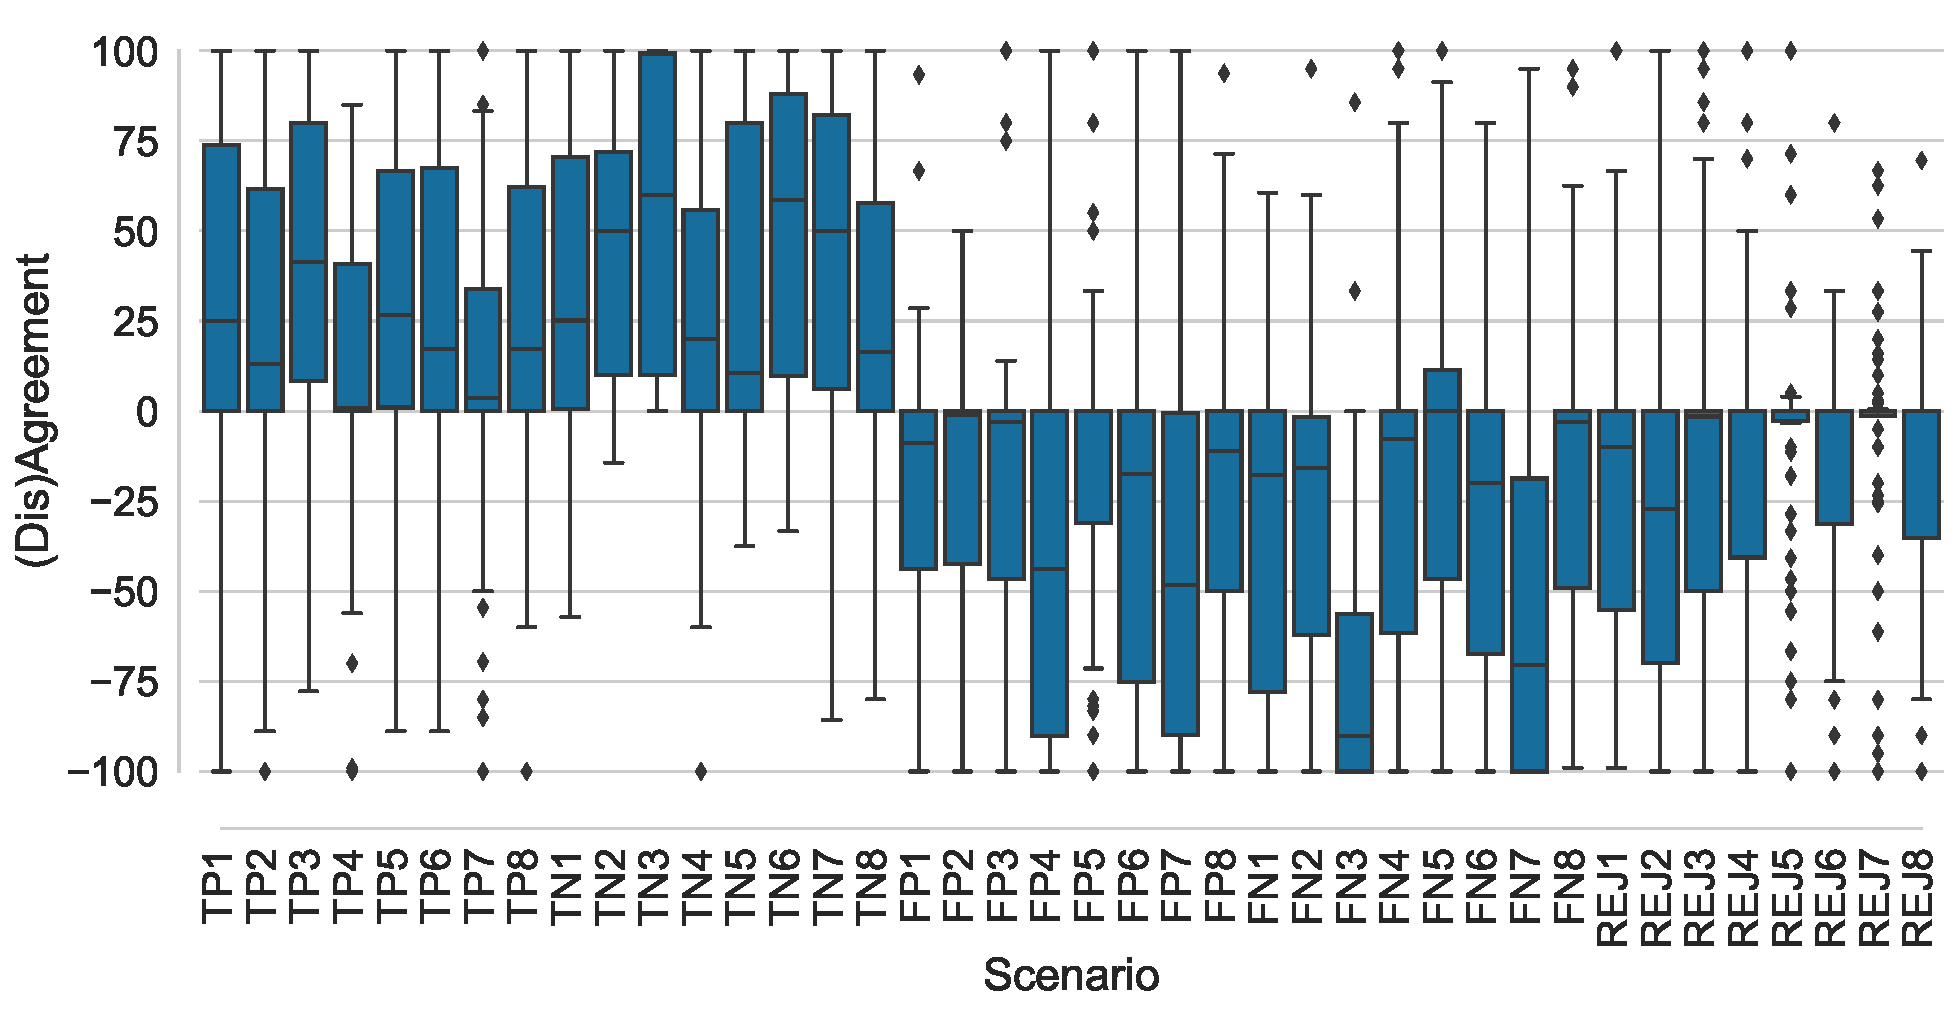
\includegraphics[width=\linewidth]{Figures/boxplots-ME.pdf}
        \caption{Scenarios rated with the ME scale.}
        \label{fig:boxplots-me}
    \end{subfigure}
    \\
    \begin{subfigure}[b]{.9\textwidth}
        \centering
        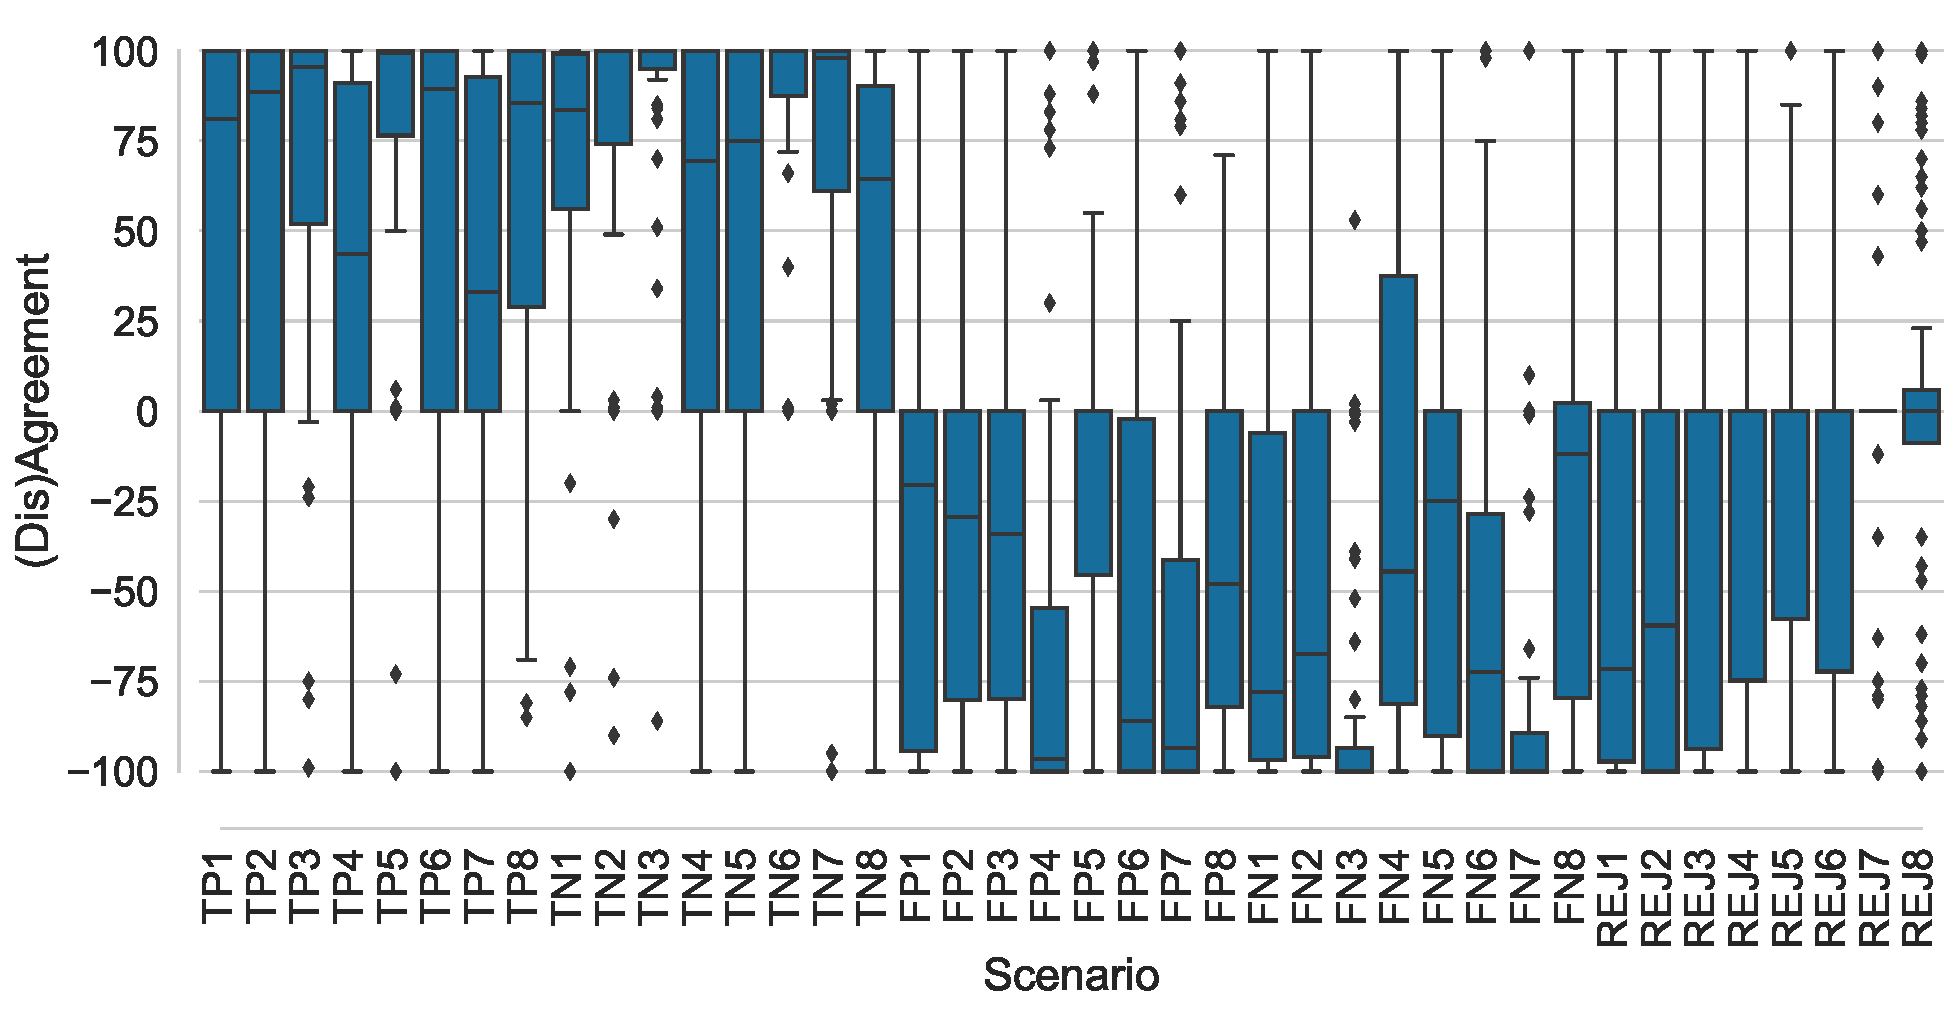
\includegraphics[width=\linewidth]{Figures/boxplots-100-level.pdf}
        \caption{Scenarios rated with the 100-level scale.}
        \label{fig:boxplots-100-level}
    \end{subfigure}
    \caption{Boxplots of the responses of all participants to all 40 scenarios.}
    \label{fig:boxplots}
\end{figure}
We calculate the value ratios by following the approach from section \ref{sec:analysis-values}.
%

%
First we calculate the median scores of all responses for each question.
%
We use the median since we found in the pilot survey that the data from both scales are highly skewed with outliers.
%
Then, we calculate the mean of all values with the same scenario type (TP, TN, FP, FN, or rejection).
%
We show the resulting value ratios in table \ref{tab:values-reliability}.
%
We

\begin{table}[t]
    \centering
    \begin{tabular}{lcccc}
        \toprule
                           & \multicolumn{2}{c}{\textbf{ME}} & \multicolumn{2}{c}{\textbf{100-level}}                                        \\
        \cmidrule(l){2-3} \cmidrule(l){4-5}
                           & $\boldsymbol{\alpha}$           & $\textbf{v}$                           & $\boldsymbol{\alpha}$ & $\textbf{v}$ \\
        \midrule
        \textbf{TP}        & 0.07                            & 18.15                                  & 0.04                  & 77.00        \\
        \textbf{TN}        & 0.10                            & 36.32                                  & 0.11                  & 86.31        \\
        \textbf{FP}        & 0.39                            & -16.69                                 & 0.07                  & -51.00       \\
        \textbf{FN}        & 0.92                            & -28.08                                 & 0.14                  & -62.43       \\
        \textbf{Rejection} & -0.31                           & -4.82                                  & 0.07                  & -16.37       \\
        \midrule
        \textbf{All}       & 0.78                            & ---                                    & 0.44                  & ---          \\
        \bottomrule
    \end{tabular}
    \caption{Krippendorff's alpha ($\alpha$) and the scenario values ($v$) for TP, TN, FP, FN, and rejection scenarios for both scales: the Magnitude Estimation (ME) and 100-level scale.}
    \label{tab:values-reliability}
\end{table}

\subsection{Reliability}
\label{sec:results-reliability}

\subsection{Validity}
\label{sec:results-validity}

\subsection{Demographics}
\label{sec:results-demographics}
\begin{table}
    \small
    \centering
    \begin{tabular}{lccc|ccc}
        \toprule
                      & \multicolumn{3}{c}{\textbf{Two groups}} & \multicolumn{3}{c}{\textbf{More than two groups}}                                                                                                                                                                       \\
        \midrule
                      & \multicolumn{1}{c}{\textbf{Sex}}        & \multicolumn{1}{c}{\textbf{Student}}              & \multicolumn{1}{c}{\textbf{Continent}} & \multicolumn{1}{c}{\textbf{Nationality}} & \multicolumn{1}{c}{\textbf{Language}}  & \multicolumn{1}{c}{\textbf{Ethnicity}} \\
        \midrule
        \textbf{TP1}  & 0.506                                   & 0.371                                             & 0.982                                  & 0.095                                    & 0.117                                  & 0.108                                  \\
        \textbf{TP2}  & 0.268                                   & 0.201                                             & 0.387                                  & 0.300                                    & 0.330                                  & 0.464                                  \\
        \textbf{TP3}  & 0.680                                   & 0.276                                             & 0.577                                  & 0.160                                    & \cellcolor[HTML]{EFEFEF}\textbf{0.046} & 0.138                                  \\
        \textbf{TP4}  & 0.756                                   & 0.441                                             & 0.774                                  & 0.137                                    & 0.175                                  & 0.568                                  \\
        \textbf{TP5}  & 0.392                                   & \cellcolor[HTML]{EFEFEF}\textbf{0.011}            & 0.387                                  & 0.152                                    & 0.106                                  & 0.341                                  \\
        \textbf{TP6}  & 0.260                                   & 0.097                                             & 0.682                                  & \cellcolor[HTML]{EFEFEF}\textbf{0.002}   & \cellcolor[HTML]{EFEFEF}\textbf{0.006} & 0.215                                  \\
        \textbf{TP7}  & 0.342                                   & 0.730                                             & 0.059                                  & 0.241                                    & 0.400                                  & 0.238                                  \\
        \textbf{TP8}  & 0.495                                   & \cellcolor[HTML]{EFEFEF}\textbf{0.015}            & 0.246                                  & 0.568                                    & 0.387                                  & 0.190                                  \\
        \textbf{TN1}  & 0.430                                   & 0.480                                             & 0.554                                  & 0.307                                    & 0.260                                  & 0.449                                  \\
        \textbf{TN2}  & 0.567                                   & 0.382                                             & 0.633                                  & 0.595                                    & 0.716                                  & 0.833                                  \\
        \textbf{TN3}  & 0.393                                   & 0.866                                             & 0.766                                  & 0.443                                    & 0.298                                  & 0.432                                  \\
        \textbf{TN4}  & 0.104                                   & 0.171                                             & 0.059                                  & 0.245                                    & 0.251                                  & 0.201                                  \\
        \textbf{TN5}  & 0.290                                   & 0.199                                             & 0.964                                  & 0.304                                    & 0.177                                  & 0.296                                  \\
        \textbf{TN6}  & 0.521                                   & 0.510                                             & 0.608                                  & 0.815                                    & 0.748                                  & 0.600                                  \\
        \textbf{TN7}  & 0.224                                   & 0.878                                             & \cellcolor[HTML]{EFEFEF}\textbf{0.050} & 0.108                                    & 0.223                                  & 0.314                                  \\
        \textbf{TN8}  & 0.191                                   & 0.417                                             & 0.327                                  & 0.168                                    & 0.761                                  & 0.872                                  \\
        \textbf{FP1}  & 0.270                                   & 0.545                                             & 0.065                                  & 0.093                                    & 0.333                                  & 0.174                                  \\
        \textbf{FP2}  & 0.337                                   & 0.114                                             & 0.155                                  & \cellcolor[HTML]{EFEFEF}\textbf{0.008}   & 0.164                                  & 0.195                                  \\
        \textbf{FP3}  & 0.561                                   & 0.509                                             & 0.889                                  & 0.793                                    & 0.725                                  & 0.205                                  \\
        \textbf{FP4}  & 0.278                                   & 0.860                                             & 0.908                                  & 0.267                                    & 0.186                                  & 0.344                                  \\
        \textbf{FP5}  & 0.847                                   & 0.445                                             & 0.220                                  & 0.269                                    & 0.554                                  & 0.194                                  \\
        \textbf{FP6}  & 0.774                                   & 0.266                                             & 0.555                                  & 0.758                                    & 0.409                                  & 0.486                                  \\
        \textbf{FP7}  & 0.391                                   & 0.784                                             & \cellcolor[HTML]{EFEFEF}\textbf{0.015} & \cellcolor[HTML]{EFEFEF}\textbf{0.026}   & \cellcolor[HTML]{EFEFEF}\textbf{0.020} & \cellcolor[HTML]{EFEFEF}\textbf{0.010} \\
        \textbf{FP8}  & 0.624                                   & 0.837                                             & 0.681                                  & 0.544                                    & 0.225                                  & 0.705                                  \\
        \textbf{FN1}  & 0.337                                   & 0.213                                             & 0.317                                  & 0.261                                    & 0.668                                  & 0.558                                  \\
        \textbf{FN2}  & 0.791                                   & 0.928                                             & 0.759                                  & 0.967                                    & 0.974                                  & 0.823                                  \\
        \textbf{FN3}  & 0.990                                   & 0.752                                             & 0.480                                  & 0.504                                    & 0.455                                  & 0.182                                  \\
        \textbf{FN4}  & 0.511                                   & 0.573                                             & 0.450                                  & 0.549                                    & 0.856                                  & 0.965                                  \\
        \textbf{FN5}  & 0.306                                   & 0.467                                             & 0.802                                  & \cellcolor[HTML]{EFEFEF}\textbf{0.001}   & \cellcolor[HTML]{EFEFEF}\textbf{0.009} & 0.349                                  \\
        \textbf{FN6}  & 0.109                                   & 0.113                                             & 0.928                                  & \cellcolor[HTML]{EFEFEF}\textbf{0.012}   & 0.084                                  & 0.436                                  \\
        \textbf{FN7}  & 0.871                                   & 0.677                                             & 0.093                                  & 0.107                                    & \cellcolor[HTML]{EFEFEF}\textbf{0.046} & 0.148                                  \\
        \textbf{FN8}  & 0.776                                   & \cellcolor[HTML]{EFEFEF}\textbf{0.009}            & 0.819                                  & 0.949                                    & 0.363                                  & 0.117                                  \\
        \textbf{REJ1} & 0.799                                   & 0.734                                             & 0.544                                  & \cellcolor[HTML]{EFEFEF}\textbf{0.021}   & \cellcolor[HTML]{EFEFEF}\textbf{0.012} & 0.168                                  \\
        \textbf{REJ2} & 0.644                                   & 0.202                                             & 0.741                                  & 0.295                                    & 0.258                                  & 0.749                                  \\
        \textbf{REJ3} & 0.803                                   & 0.815                                             & 0.108                                  & 0.425                                    & 0.482                                  & 0.133                                  \\
        \textbf{REJ4} & 0.985                                   & 1.000                                             & \cellcolor[HTML]{EFEFEF}\textbf{0.002} & \cellcolor[HTML]{EFEFEF}\textbf{0.014}   & \cellcolor[HTML]{EFEFEF}\textbf{0.036} & \cellcolor[HTML]{EFEFEF}\textbf{0.002} \\
        \textbf{REJ5} & 0.133                                   & 0.994                                             & 0.570                                  & 0.111                                    & \cellcolor[HTML]{EFEFEF}\textbf{0.036} & 0.090                                  \\
        \textbf{REJ6} & 0.244                                   & 0.195                                             & 0.716                                  & 0.061                                    & 0.166                                  & 0.664                                  \\
        \textbf{REJ7} & 0.911                                   & 0.853                                             & 0.942                                  & 0.997                                    & 0.996                                  & \cellcolor[HTML]{EFEFEF}\textbf{0.020} \\
        \textbf{REJ8} & 0.157                                   & 0.167                                             & 0.944                                  & 0.901                                    & 0.741                                  & 0.108                                  \\
        \bottomrule
    \end{tabular}
    \caption{\textbf{Individual}: an overview of the statistical differences between different groups of participants for various demographic characteristics for each scenario in the ME survey. Each cell contains the p value of either the Mann-Whitney U test for two groups or the Kruskal-Wallis test for more than two groups. The grey cells with bold text indicate significant statistical differences between the groups for that feature and scenario type.}
    \label{tab:results-differences-ind}
\end{table}

\begin{table}
    \small
    \centering
    \begin{tabular}{lccc|ccc}
        \toprule
                     & \multicolumn{3}{c}{\textbf{Two groups}} & \multicolumn{3}{c}{\textbf{More than two groups}}                                                                                                                                                                       \\
        \midrule
                     & \multicolumn{1}{c}{\textbf{Sex}}        & \multicolumn{1}{c}{\textbf{Student}}              & \multicolumn{1}{c}{\textbf{Continent}} & \multicolumn{1}{c}{\textbf{Nationality}} & \multicolumn{1}{c}{\textbf{Language}}  & \multicolumn{1}{c}{\textbf{Ethnicity}} \\
        \midrule
        \textbf{TP}  & 0.302                                   & \cellcolor[HTML]{EFEFEF}\textbf{0.032}            & 0.286                                  & 0.218                                    & 0.109                                  & 0.242                                  \\
        \textbf{TN}  & 0.726                                   & 0.379                                             & 0.204                                  & 0.190                                    & 0.216                                  & 0.281                                  \\
        \textbf{FP}  & 0.699                                   & 0.933                                             & 0.073                                  & \cellcolor[HTML]{EFEFEF}\textbf{0.020}   & \cellcolor[HTML]{EFEFEF}\textbf{0.040} & \cellcolor[HTML]{EFEFEF}\textbf{0.037} \\
        \textbf{FN}  & 0.961                                   & 0.150                                             & 0.847                                  & 0.478                                    & 0.438                                  & 0.584                                  \\
        \textbf{REJ} & 0.835                                   & 0.625                                             & 0.496                                  & 0.271                                    & 0.103                                  & 0.068                                  \\
        \bottomrule
    \end{tabular}
    \caption{\textbf{Aggregated}: an overview of the statistical differences between different groups of participants for various demographic characteristics for each aggregated scenario type in the ME survey. Each cell contains the p value of either the Mann-Whitney U test for two groups or the Kruskal-Wallis test for more than two groups. The grey cells with bold text indicate significant statistical differences between the groups for that feature and scenario type.}
    \label{tab:results-differences-grp}
\end{table}

\begin{table}
    \scriptsize
    \centering
    \setlength\tabcolsep{2pt}
    \begin{subtable}{.44\textwidth}
        \centering
        \begin{tabular}{lcccc}
            \toprule
                                  & \textbf{South Africa} & \textbf{Poland}                        & \textbf{Portugal} & \textbf{Spain} \\
            \midrule
            \textbf{South Africa} & 1.000                 &                                        &                   &                \\
            \textbf{Poland}       & 0.077                 & 1.000                                  &                   &                \\
            \textbf{Portugal}     & 0.077                 & \cellcolor[HTML]{EFEFEF}\textbf{0.009} & 1.000             &                \\
            \textbf{Spain}        & 0.119                 & 0.083                                  & 0.613             & 1.000          \\
            \bottomrule
        \end{tabular}
        \caption{TP6}
    \end{subtable}%
    \begin{subtable}{.44\textwidth}
        \centering
        \begin{tabular}{cccc}
            \toprule
            \textbf{South Africa}                  & \textbf{Poland}                        & \textbf{Portugal}                      & \textbf{Spain} \\
            \midrule
            1.000                                  &                                        &                                        &                \\
            0.755                                  & 1.000                                  &                                        &                \\
            0.261                                  & 0.261                                  & 1.000                                  &                \\
            \cellcolor[HTML]{EFEFEF}\textbf{0.026} & \cellcolor[HTML]{EFEFEF}\textbf{0.038} & \cellcolor[HTML]{EFEFEF}\textbf{0.050} & 1.000          \\
            \bottomrule
        \end{tabular}
        \caption{FP2}
    \end{subtable}
    \vskip\baselineskip
    \begin{subtable}{.44\textwidth}
        \centering
        \begin{tabular}{lcccc}
            \toprule
                                  & \textbf{South Africa}                  & \textbf{Poland} & \textbf{Portugal} & \textbf{Spain} \\
            \midrule
            \textbf{South Africa} & 1.000                                  &                 &                   &                \\
            \textbf{Poland}       & 0.342                                  & 1.000           &                   &                \\
            \textbf{Portugal}     & 0.304                                  & 1.000           & 1.000             &                \\
            \textbf{Spain}        & \cellcolor[HTML]{EFEFEF}\textbf{0.043} & 0.304           & 0.220             & 1.000          \\
            \bottomrule
        \end{tabular}
        \caption{FP7}
    \end{subtable}%
    \begin{subtable}{.44\textwidth}
        \centering
        \begin{tabular}{cccc}
            \toprule
            \textbf{South Africa}                  & \textbf{Poland}                        & \textbf{Portugal} & \textbf{Spain} \\
            \midrule
            1.000                                  &                                        &                   &                \\
            \cellcolor[HTML]{EFEFEF}\textbf{0.034} & 1.000                                  &                   &                \\
            0.150                                  & \cellcolor[HTML]{EFEFEF}\textbf{0.011} & 1.000             &                \\
            \cellcolor[HTML]{EFEFEF}\textbf{0.045} & \cellcolor[HTML]{EFEFEF}\textbf{0.011} & 0.679             & 1.000          \\
            \bottomrule
        \end{tabular}
        \caption{FN5}
    \end{subtable}
    \vskip\baselineskip
    \begin{subtable}{.44\textwidth}
        \centering
        \begin{tabular}{lcccc}
            \toprule
                                  & \textbf{South Africa} & \textbf{Poland} & \textbf{Portugal} & \textbf{Spain} \\
            \midrule
            \textbf{South Africa} & 1.000                 &                 &                   &                \\
            \textbf{Poland}       & 0.095                 & 1.000           &                   &                \\
            \textbf{Portugal}     & 0.622                 & 0.095           & 1.000             &                \\
            \textbf{Spain}        & 0.104                 & 0.095           & 0.104             & 1.000          \\
            \bottomrule
        \end{tabular}
        \caption{FN6}
    \end{subtable} %
    \begin{subtable}{.44\textwidth}
        \centering
        \begin{tabular}{cccc}
            \toprule
            \textbf{South Africa} & \textbf{Poland} & \textbf{Portugal} & \textbf{Spain} \\
            \midrule
            1.000                 &                 &                   &                \\
            0.088                 & 1.000           &                   &                \\
            0.227                 & 0.088           & 1.000             &                \\
            1.000                 & 0.227           & 0.388             & 1.000          \\
            \bottomrule
        \end{tabular}
        \caption{REJ1}
    \end{subtable}%
    \vskip\baselineskip
    \begin{subtable}{.44\textwidth}
        \centering
        \begin{tabular}{lcccc}
            \toprule
                                  & \textbf{South Africa} & \textbf{Poland} & \textbf{Portugal} & \textbf{Spanish} \\
            \midrule
            \textbf{South Africa} & 1.000                 &                 &                   &                  \\
            \textbf{Poland}       & 0.098                 & 1.000           &                   &                  \\
            \textbf{Portugal}     & 0.098                 & 1.000           & 1.000             &                  \\
            \textbf{Spain}        & 0.098                 & 0.422           & 0.422             & 1.000            \\
            \bottomrule
        \end{tabular}
        \caption{REJ4}
    \end{subtable}
    \caption{\textbf{Nationality}: an overview of all pairwise Mann-Whitney U tests between the different nationalities for all scenarios where we found significant differences between all nationalities using the Kruskal-Wallis test. Each cell contains the p value of the Mann-Whitney U test between two groups of different nationalities. We corrected all p values with the Benjamini-Hochberg procedure. The grey cells with bold text indicate significant statistical differences between the two nationalities.}
\end{table}

\begin{table}
    \scriptsize
    \centering
    \setlength\tabcolsep{2pt}
    \begin{subtable}{.405\textwidth}
        \centering
        \begin{tabular}{lcccc}
            \toprule
                               & \textbf{English} & \textbf{Polish} & \textbf{Portugese} & \textbf{Spanish} \\
            \midrule
            \textbf{English}   & 1.000            &                 &                    &                  \\
            \textbf{Polish}    & 0.561            & 1.000           &                    &                  \\
            \textbf{Portugese} & 0.352            & 0.283           & 1.000              &                  \\
            \textbf{Spanish}   & 0.176            & 0.258           & 0.142              & 1.000            \\
            \bottomrule
        \end{tabular}
        \caption{TP3}
    \end{subtable}%
    \begin{subtable}{.405\textwidth}
        \centering
        \begin{tabular}{cccc}
            \toprule
            \multicolumn{1}{c}{\textbf{English}} & \multicolumn{1}{c}{\textbf{Polish}}    & \textbf{Portugese} & \textbf{Spanish} \\
            \midrule
            1.000                                & \multicolumn{1}{c}{}                   &                    &                  \\
            0.089                                & 1.000                                  &                    &                  \\
            0.119                                & \cellcolor[HTML]{EFEFEF}\textbf{0.007} & 1.000              &                  \\
            0.522                                & 0.089                                  & 1.000              & 1.000            \\
            \bottomrule
        \end{tabular}
        \caption{TP6}
    \end{subtable}
    \vskip\baselineskip
    \begin{subtable}{.405\textwidth}
        \centering
        \begin{tabular}{lcccc}
            \toprule
                               & \textbf{English}                       & \textbf{Polish} & \textbf{Portugese} & \textbf{Spanish} \\
            \midrule
            \textbf{English}   & 1.000                                  &                 &                    &                  \\
            \textbf{Polish}    & 0.321                                  & 1.000           &                    &                  \\
            \textbf{Portugese} & 0.321                                  & 1.000           & 1.000              &                  \\
            \textbf{Spanish}   & \cellcolor[HTML]{EFEFEF}\textbf{0.019} & 0.444           & 0.321              & 1.000            \\
            \bottomrule
        \end{tabular}
        \caption{FP7}
    \end{subtable}%
    \begin{subtable}{.405\textwidth}
        \centering
        \begin{tabular}{cccc}
            \toprule
            \textbf{English} & \textbf{Polish}                        & \textbf{Portugese} & \textbf{Spanish} \\
            \midrule
            1.000            &                                        &                    &                  \\
            0.070            & 1.000                                  &                    &                  \\
            0.209            & \cellcolor[HTML]{EFEFEF}\textbf{0.011} & 1.000              &                  \\
            0.647            & 0.164                                  & 0.838              & 1.000            \\
            \bottomrule
        \end{tabular}
        \caption{FN5}
    \end{subtable}
    \vskip\baselineskip
    \begin{subtable}{.405\textwidth}
        \centering
        \begin{tabular}{lcccc}
            \toprule
                               & \textbf{English}                       & \textbf{Polish} & \textbf{Portugese} & \textbf{Spanish} \\
            \midrule
            \textbf{English}   & 1.000                                  &                 &                    &                  \\
            \textbf{Polish}    & 0.895                                  & 1.000           &                    &                  \\
            \textbf{Portugese} & 0.439                                  & 0.721           & 1.000              &                  \\
            \textbf{Spanish}   & \cellcolor[HTML]{EFEFEF}\textbf{0.049} & 0.309           & 0.548              & 1.000            \\
            \bottomrule
        \end{tabular}
        \caption{FN7}
    \end{subtable}%
    \begin{subtable}{.405\textwidth}
        \centering
        \begin{tabular}{cccc}
            \toprule
            \textbf{English} & \textbf{Polish} & \textbf{Portugese} & \textbf{Spanish} \\
            \midrule
            1.000            &                 &                    &                  \\
            0.076            & 1.000           &                    &                  \\
            0.387            & 0.076           & 1.000              &                  \\
            0.149            & 0.711           & 0.096              & 1.000            \\
            \bottomrule
        \end{tabular}
        \caption{REJ1}
    \end{subtable}
    \vskip\baselineskip
    \begin{subtable}{.405\textwidth}
        \centering
        \begin{tabular}{lcccc}
            \toprule
                               & \textbf{English} & \textbf{Polish} & \textbf{Portugese} & \textbf{Spanish} \\
            \midrule
            \textbf{English}   & 1.000            &                 &                    &                  \\
            \textbf{Polish}    & 0.063            & 1.000           &                    &                  \\
            \textbf{Portugese} & 0.063            & 1.000           & 1.000              &                  \\
            \textbf{Spanish}   & 0.599            & 1.000           & 1.000              & 1.000            \\
            \bottomrule
        \end{tabular}
        \caption{REJ4}
    \end{subtable}%
    \begin{subtable}{.405\textwidth}
        \centering
        \begin{tabular}{cccc}
            \toprule
            \textbf{English} & \textbf{Polish} & \textbf{Portugese} & \textbf{Spanish} \\
            \midrule
            1.000            &                 &                    &                  \\
            1.000            & 1.000           &                    &                  \\
            0.489            & 0.452           & 1.000              &                  \\
            0.105            & 0.152           & 0.105              & 1.000            \\
            \bottomrule
        \end{tabular}
        \caption{REJ5}
    \end{subtable}
    \caption{\textbf{Language}: an overview of all pairwise Mann-Whitney U tests between the different spoken languages for all scenarios where we found significant differences between all spoken languages using the Kruskal-Wallis test. Each cell contains the p value of the Mann-Whitney U test between two groups of languages. We corrected all p values with the Benjamini-Hochberg procedure. The grey cells with bold text indicate significant statistical differences between the two languages.}
\end{table}

\begin{table}
    \scriptsize
    \centering
    \setlength\tabcolsep{2pt}
    \begin{subtable}{.275\textwidth}
        \centering
        \begin{tabular}{lccc}
            \toprule
                           & \textbf{White}                         & \textbf{Mixed}                         & \textbf{Black} \\
            \midrule
            \textbf{White} & 1.000                                  &                                        &                \\
            \textbf{Mixed} & 0.552                                  & 1.000                                  &                \\
            \textbf{Black} & \cellcolor[HTML]{EFEFEF}\textbf{0.028} & \cellcolor[HTML]{EFEFEF}\textbf{0.028} & 1.000          \\
            \bottomrule
        \end{tabular}
        \caption{FP7}
    \end{subtable}%
    \begin{subtable}{.21\textwidth}
        \centering
        \begin{tabular}{ccc}
            \toprule
            \multicolumn{1}{l}{\textbf{White}}     & \textbf{Mixed}                                             & \textbf{Black}            \\
            \midrule
            1.000                                  &                                                            &                           \\
            0.776                                  & \multicolumn{1}{r}{1.000}                                  &                           \\
            \cellcolor[HTML]{EFEFEF}\textbf{0.002} & \multicolumn{1}{r}{\cellcolor[HTML]{EFEFEF}\textbf{0.776}} & \multicolumn{1}{r}{1.000} \\
            \bottomrule
        \end{tabular}
        \caption{REJ4}
    \end{subtable}%
    \begin{subtable}{.21\textwidth}
        \centering
        \begin{tabular}{ccc}
            \toprule
            \multicolumn{1}{l}{\textbf{White}}     & \textbf{Mixed}            & \textbf{Black}            \\
            \midrule
            1.000                                  &                           &                           \\
            \cellcolor[HTML]{EFEFEF}\textbf{0.016} & \multicolumn{1}{r}{1.000} &                           \\
            1.000                                  & \multicolumn{1}{r}{0.112} & \multicolumn{1}{r}{1.000} \\
            \bottomrule
        \end{tabular}
        \caption{REJ7}
    \end{subtable}
    \caption{\textbf{Ethnicity}: an overview of all pairwise Mann-Whitney U tests between the different ethnicities for all scenarios where we found significant differences between all ethnicities using the Kruskal-Wallis test. Each cell contains the p value of the Mann-Whitney U test between two groups of ethnicities. We corrected all p values with the Benjamini-Hochberg procedure. The grey cells with bold text indicate significant statistical differences between the two ethnicities.}
\end{table}

\section{Value-sensitive rejection}
\label{sec:results-rejector}
\todo[inline]{Explain that the metric conditions still hold if we set $V_{tp}$ and $V_{tn}$ to 0}
